
%% ========================================================================
%%%% Document settings
%% ========================================================================

%% Document class with actual values
\documentclass[parskip=half,BCOR=0mm,oneside]{scrbook}

%% Custom commands (moved after \documentclass)
\newcommand{\myparskip}{half}
\newcommand{\myBCOR}{0mm}
\newcommand{\mylaterality}{oneside}
\newcommand{\mydispositioncolor}{22,72,154}
\newcommand{\mylinespread}{1.5}
\newcommand{\mycolorlinks}{false}  %% "true" or "false"
\newcommand{\mylanguage}{american,ngerman}


%% ========================================================================
%%%% Document metadata
%% ========================================================================

%% Student:
\newcommand{\myauthor}{Linus Baumann, Alexander Dixon, Cosima Dotzauer, Dennis Hilgert, Jonas Werner}
\newcommand{\myhomestreet}{Berggasse 16}
\newcommand{\myhomepostalnumber}{67269}
\newcommand{\myhometown}{Grünstadt}
\newcommand{\myid}{xxxxxxx, xxxxxxx, 3750882, xxxxxxx, xxxxxxx}

%% Titel und PDF-Einstellungen
\newcommand{\myworktype}{Laborabeit}
\newcommand{\mytitle}{Entwicklung einer Cloud Native App}
\newcommand{\mysubtitle}{ }
\newcommand{\mysubject}{Laborarbeit}
\newcommand{\mykeywords}{Key, Word}


%% Dualer Partner
\newcommand{\mydualpartner}{}
%% Duale Hochschule
\newcommand{\myuniversity}{DHBW-CAS}
\newcommand{\mystudy}{Informatik}
\newcommand{\myevaluator}{Prof. Dr. Christoph Sturm}
\newcommand{\mysemester}{SoSe 2025}
\newcommand{\mycourse}{W3M20035}
\newcommand{\myworktitle}{in Cloud Infrastructures and Cloud Native Applications}
%% Datum
\newcommand{\mysubmissionday}{28}
\newcommand{\mysubmissionmonth}{September}
\newcommand{\mysubmissionyear}{2025}


%% ========================================================================
%%%% Other settings
%% ========================================================================

%% !!FIRST!! Load preamble

% set raggedbottom if \mylaterality is 'twoside' to prevent weird spaces between text blocks
\makeatletter
\if@twoside%
    \raggedbottom
\fi%  
\makeatother

%% Set paper and border size
\usepackage[paper=a4paper,left=25mm,right=25mm,top=25mm,bottom=25mm]{geometry}

%% UTF8 as input characters; UCS incompatible to biblatex
\usepackage[utf8]{inputenc}

%% The default setting of the language is American. Please change settings for
%% additional or alternative languages used in main.tex.
%% Please note that the default language of the document is the *last* language
%% which is added to the package options.
%% To set only parts of your document in a different language as the rest,
%% use for example\newline\verb+\foreignlanguage{ngerman}{Beispieltext in deutscher Sprache}+\newline
\usepackage[\mylanguage]{babel}

%% This package defines basic colors. If you want to get rid of colored links
%% and headings please change corresponding value in main.tex to {0,0,0}.
%% Used for links and so forth in screen-version
\usepackage[usenames,dvipsnames]{xcolor}
\definecolor{DispositionColor}{RGB}{\mydispositioncolor}

%% The widely used package to use graphical images within a LaTeX document.
%% \includegraphics[width=42mm]{figures/image}
\usepackage[pdftex]{graphicx}
%%package to include a graphik with text under it
\usepackage{float}

%% For example on title pages you might want to have a logo on the upper right
%% corner of the first page (only). The package \texttt{eso-pic} is able to
%% place things on absolute and relative positions on the whole page.
\usepackage{eso-pic}

%% List of abbreviations
\usepackage[printonlyused]{acronym}
\usepackage{patchcmd}

%% Use biblatex for bibliography
%% With "Sorting=None" the numbering is done according to the order of appearance. 
\usepackage[style=numeric,sorting=none]{biblatex}
%% Used for quotes (loaded later after minted)
% \usepackage{csquotes}

%% Add fontec to hyphenate umlaut and fix-cm to fix changes in section heading
\usepackage[T1]{fontenc}
\usepackage{fix-cm}

%% Use caption package before minitoc; no KOMA option to avoid errors
\usepackage{caption}
\captionsetup{font={footnotesize,sf},labelfont={footnotesize,bf}}
%% Produce a table of contents for each chapter, part or section
\usepackage{minitoc}
%% Add default bibliography
\addbibresource{etc/literature.bib}

%% Give name to bibliography
\bibliography{Literaturverzeichnis}

%% ========================================================================
%%%% Typographic settings
%% ========================================================================

%% If you have to enlarge the distance between two lines of text, you can
%% increase it using the \texttt{\mylinespread} command in \texttt{main.tex}. By default, it is
%% deactivated (set to 100~percent). Modify only with caution since it influences the
%% page layout and could lead to ugly looking documents.
\linespread{\mylinespread}

\renewcommand*{\chapterheadstartvskip}{\vspace*{0\baselineskip}}% Abstand einstellen

%% Reduce space between section and chapter headings
\RedeclareSectionCommand[
   beforeskip=0pt,
   afterskip=1sp
]{chapter}

\RedeclareSectionCommand[
   beforeskip=0pt,
   afterskip=1sp
]{section}

\RedeclareSectionCommand[
   beforeskip=0pt,
   afterskip=1sp
]{subsection}

\RedeclareSectionCommand[
   beforeskip=0pt,
   afterskip=1sp
]{subsubsection}

%% This document template is able to generate an output that uses colorized
%% headings, captions, page numbers, and links. The color named
%% `DispositionColor' used in this document is defined near the definition
%% of package xcolor
%% The changes required for headings, page numbers and captions are defined
%% here.
%% Settings for colored links are handled by the definitions of the
%% hyperref package
%% \setheadsepline{.4pt}[\color{DispositionColor}]
\renewcommand{\headfont}{\normalfont\sffamily\color{DispositionColor}}
\renewcommand{\pnumfont}{\normalfont\sffamily\color{DispositionColor}}
\addtokomafont{disposition}{\color{DispositionColor}}
\addtokomafont{caption}{\color{DispositionColor}\footnotesize}
\addtokomafont{captionlabel}{\color{DispositionColor}}


%% Add package to add long text tables
\usepackage{longtable}
\usepackage{booktabs}
\usepackage{colortbl}
%% ========================================================================
%%%% Source code highlighting
%% ========================================================================

%% Minted for source code highlighting
\usepackage[newfloat]{minted}

%%\BeforeBeginEnvironment{minted}{\medskip}
%%\AfterEndEnvironment{minted}{\smallskip}

%% Define background color for style "friendly"
\definecolor{friendlybg}{HTML}{f0f0f0}

%% Settings for source code
\definecolor{codebg}{rgb}{0.95,0.95,0.95}
\setminted{
    bgcolor=codebg,
    startinline=true,
    obeytabs=true,
    tabsize=4,
    linenos,
    breaklines,
    fontsize=\small,
    baselinestretch=1.2,
    samepage=true
}

\renewcommand{\listingname}{Auflistung}

%% Load csquotes after fvextra/minted to avoid warnings
\usepackage{csquotes}


\usepackage{etoolbox}

\makeatletter
\AtBeginEnvironment{minted}{\dontdofcolorbox}
\def\dontdofcolorbox{\renewcommand\fcolorbox[4][]{##4}}
\makeatother

%% for the code-block environment with listing and reference possibility:
%% \begin{code}{<language>}{<caption>}{<label>} 
%% ... 
%% \end{code}
%% is also used with minted so there is a list of code blocks
% listings removed to avoid clash with minted/newfloat 'listing' float
\usepackage[figure,table,listing]{totalcount}
%% Caption settings for minted 'listing' float
\captionsetup[listing]{skip=5pt,belowskip=15pt} % spacing for the label
%% the following see also here: https://github.com/gpoore/minted/issues/108
\newcommand{\storeCaption}{}
\newcommand{\storeLabel}{}
\newenvironment{codelisting}{\captionsetup{type=listing}}{}
\newenvironment{code}[3]
{%
	\VerbatimEnvironment
	\renewcommand{\storeCaption}{#2}%
	\renewcommand{\storeLabel}{#3}%
	\begin{minipage}{\linewidth}%
	\begin{codelisting}%
	\begin{minted}{#1}%
	}
	{%
	\end{minted}%
	\caption{%
	    {
	    \setmintedinline{fontsize=\footnotesize}%
	    \storeCaption %
	    }%
    	}%
	\label{\storeLabel}%
	\end{codelisting}%
	\end{minipage}%
}

% caption is already loaded with KOMA integration above; avoid duplicate loads

%%Packages for Pseudoalgorithm
\usepackage{algorithm} 
\usepackage{algpseudocode} 

%\hyphenation{Get-Stream-With-Image-Rotated-For-External-Storage ab-hör-si-cher-en Funk-ti-ons-um-fang Dev-EUI Bild-er-ken-nung}

%% !!LAST!! Do PDF settings
%% ========================================================================
%%%% PDF settings
%% ========================================================================

\pdfcompresslevel=9

%% Declarations of hyperref should be the last definitions of the preamble
\usepackage[
unicode=true,
backref,
pagebackref=false,
bookmarks=true,
bookmarksopen=false,
pdfpagemode=UseNone,
plainpages=false,
urlcolor=DispositionColor,
linkcolor=DispositionColor,
citecolor=DispositionColor,
anchorcolor=DispositionColor,
colorlinks=\mycolorlinks,
breaklinks
]{hyperref}

%% all strings need to be loaded after hyperref was loaded with unicode support
%% if not the field is garbled in the output for characters like ČŽĆŠĐ
\hypersetup{
pdftitle = {\mytitle},
pdfauthor = {\myauthor},
pdfsubject = {\mysubject},
pdfproducer = {\myauthor},
pdfkeywords = {\mykeywords}
}

%% Break URLs in bibliography
\PassOptionsToPackage{hyphens}{url}
\setcounter{biburllcpenalty}{8000}
%% ========================================================================
%%%% begin{document}
%% ========================================================================
\usepackage{tikz}
\begin{document}
\sffamily
\frontmatter

%% Titelseite
%% Layout mit Firmen und DHBW Angaben
%% ========================================================================
%%%% Information
%% ========================================================================
%% Titelseite für Arbeiten mit der dualen Hochschule Mosbach und dem
%% Unternehmen WIKA.
%% Die anzuzeigenden Daten werden in der Datei main.tex festgelegt.

\begin{titlepage}
%% Company Logo
\AddToShipoutPicture*{
    \AtPageUpperLeft{
        \hspace{\paperwidth}
        \raisebox{-50mm}{
            \makebox[-129mm][r]{
\includegraphics[width=50mm]{template/figures/University_Logo}}
        }
    }
}
%% University Logo
\AddToShipoutPicture*{
    \AtPageUpperLeft{
        \hspace{\paperwidth}
        \raisebox{-50mm}{
            \makebox[-39mm][r]{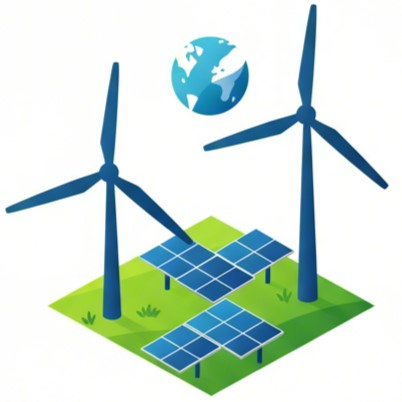
\includegraphics[width=30mm]{template/figures/Company_Logo}}
        }
    }
}


\begin{center}
~
\vfill\vfill\vfill \vfill\vfill

\sffamily

{\LARGE\bfseries\mytitle}

{\large\bfseries\mysubtitle}

\vfill\vfill
{\normalsize\bfseries\myworktype~\myworktitle}\\

\vfill \vfill
Im Master Studiengang \mystudy ~an der\\
{\normalsize\bfseries\myuniversity}

\vfill
von\\
\myauthor

\vfill
\mysubmissionday. \mysubmissionmonth~\mysubmissionyear

\vfill\vfill\vfill
\end{center}

\sffamily{
\begin{tabular}{ll}
    Matrikelnummern & \myid \\
    Kurs & \mycourse \\
    Semester & \mysemester \\
    Begutachter & \myevaluator \\
\end{tabular}
}

\end{titlepage}

\newpage

%% Verwendung von Projekt-Deckblatt
%%%% ========================================================================
%%%% Information
%% ========================================================================
%% Titelseite für Arbeiten mit der dualen Hochschule Mosbach und dem
%% Unternehmen WIKA.
%% Die anzuzeigenden Daten werden in der Datei main.tex festgelegt.

\begin{titlepage}

%% Company Logo
\AddToShipoutPicture*{
    \AtPageUpperLeft{
        \hspace{\paperwidth}
        \raisebox{-50mm}{
            \makebox[-129mm][r]{
\includegraphics[width=42mm]{template/figures/DHBW.png}}
        }
    }
}

%% University Logo
\AddToShipoutPicture*{
    \AtPageUpperLeft{
        \hspace{\paperwidth}
        \raisebox{-52mm}{
            \makebox[-129mm][r]{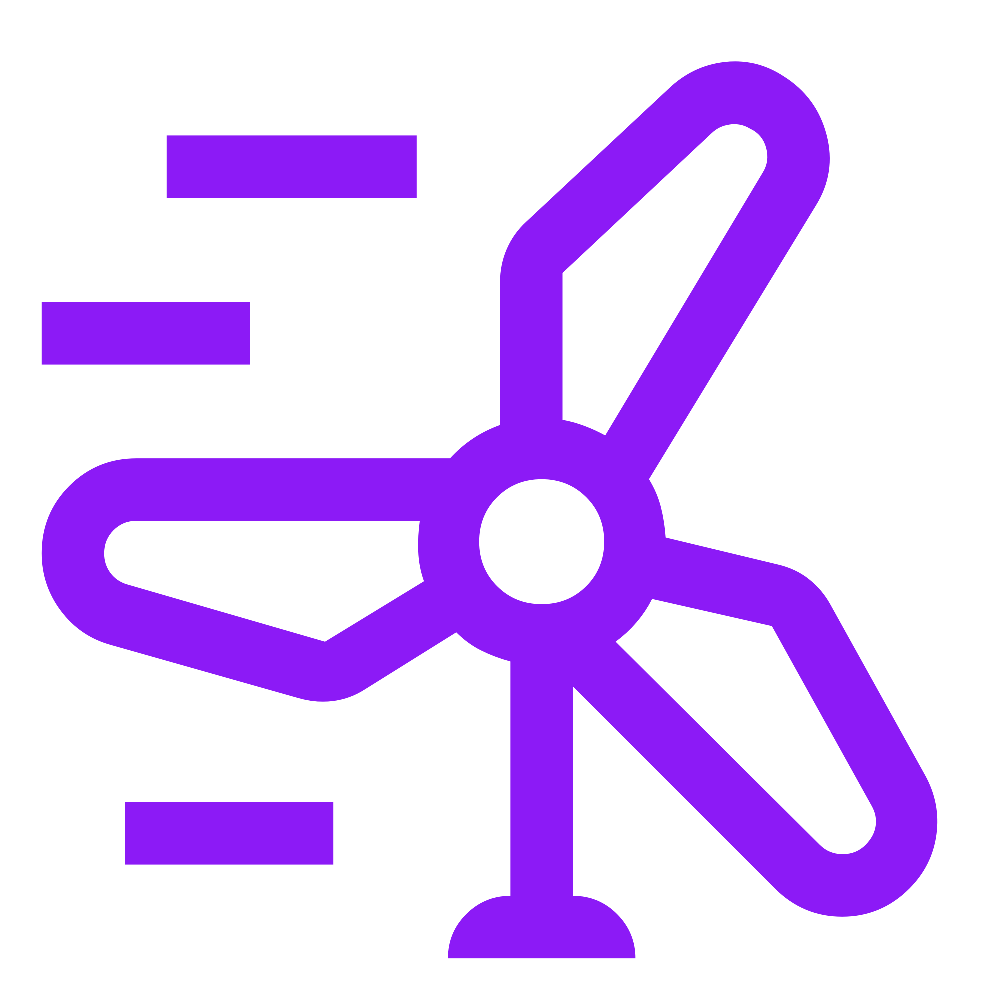
\includegraphics[width=25mm]{template/figures/Company_Logo.png}}
        }
    }
}

\begin{center}
~
\vfill\vfill\vfill \vfill\vfill

\sffamily

{\LARGE\bfseries\mytitle}

{\large\bfseries\mysubtitle}

\vfill\vfill
{\normalsize\bfseries\myworktype~\myworktitle}\\

\vfill \vfill
Im Studiengang \mystudy\\
an der \myuniversity

\vfill
von\\
\textbf{\myauthor}

\vfill
\mysubmissionday. \mysubmissionmonth~\mysubmissionyear

\vfill\vfill\vfill
\end{center}

\sffamily{
\begin{tabular}{ll}
    Matrikelnummer & \myid \\
    Ausbildungsfirma & \mydualpartner \\
    & \mydualpartnerLocation \\
    Betreuer der Ausbildungsfirma & \mysupervisor \\
\end{tabular}
}

\end{titlepage}

\newpage

%% Verwendung von Projekt-Deckblatt
%% %% ========================================================================
%%%% Information
%% ========================================================================
%% Titelseite für Arbeiten mit der dualen Hochschule Mosbach und dem
%% Unternehmen WIKA.
%% Die anzuzeigenden Daten werden in der Datei main.tex festgelegt.

\begin{titlepage}

%% Company Logo
\AddToShipoutPicture*{
    \AtPageUpperLeft{
        \hspace{\paperwidth}
        \raisebox{-50mm}{
            \makebox[-129mm][r]{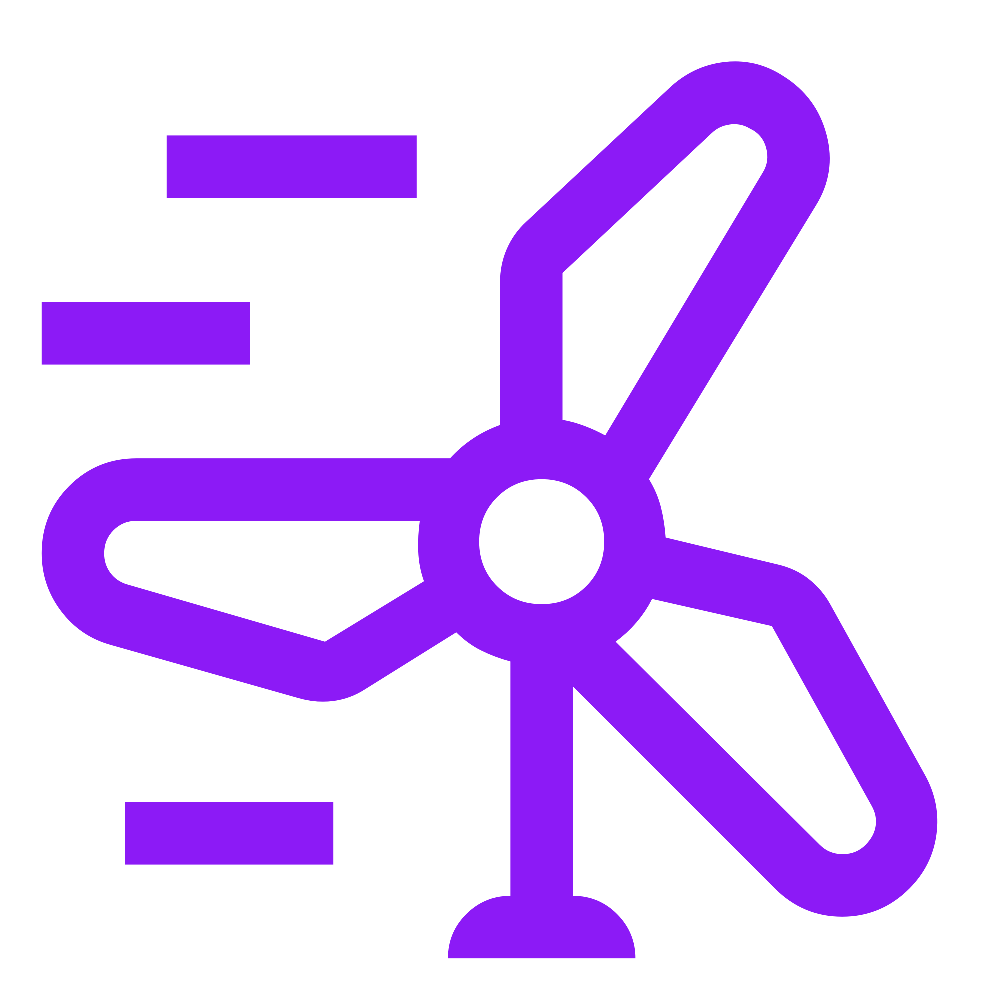
\includegraphics[width=42mm]{template/figures/Company_Logo.png}}
        }
    }
}

%% University Logo
\AddToShipoutPicture*{
    \AtPageUpperLeft{
        \hspace{\paperwidth}
        \raisebox{-52mm}{
            \makebox[-39mm][r]{
\includegraphics[width=42mm]{template/figures/DHBW.png}}
        }
    }
}

\begin{center}
~
\vfill\vfill\vfill \vfill\vfill

\sffamily

{\LARGE\bfseries\mytitle}

{\large\bfseries\mysubtitle}

\vfill\vfill
{\normalsize\bfseries\ BACHELORARBEIT}\\

\vfill\vfill
für die Prüfung zum \\
\mydegree

\vfill \vfill
des Studiengangs \mystudy\\
an der \myuniversity

\vfill
von\\
\textbf{\myauthor}

\vfill
\mysubmissionday. \mysubmissionmonth~\mysubmissionyear

\vfill\vfill\vfill
\end{center}

\sffamily{
\begin{tabular}{ll}
    Bearbeitungszeitraum & 12 Wochen \\
    Matrikelnummer, Kurs & \myid, \mycourse \\
    Ausbildungsfirma & \mydualpartner, \mydualpartnerLocation \\
    Betreuer der Ausbildungsfirma & \mysupervisor \\
    Gutachter der Dualen Hochschule & \myevaluator
\end{tabular}
}

\end{titlepage}

\newpage


%% Sperrvermerk
%% %% Sperrvermerk
\section*{Sperrvermerk}
Die vorgelegte \myworktype ~mit dem Titel \glqq\textit{{\mytitle}}\grqq{} beinhaltet vertrauliche Informationen und Daten des Unternehmens \mydualpartner.

Diese \myworktype ~darf nur vom Erst- und Zweitgutachter sowie berechtigten Mitgliedern des Prüfungsausschusses eingesehen werden. Eine Vervielfältigung und Veröffentlichung der \myworktype ~ist auch auszugsweise nicht erlaubt.

Dritten darf diese Arbeit nur mit der ausdrücklichen Genehmigung des Verfassers und Unternehmens zugänglich gemacht werden.

\newpage
%% Eidesstattliche Erklärung
%% %% Neuen Befehl für Textfelder definieren
\newcommand{\textfield}[2]{
    \vbox{
        \hsize=#1\kern3cm\hrule\kern1ex
        \hbox to \hsize{\strut\hfil\footnotesize#2\hfil}
    }
}

%% Eidesstattliche Erklärung
\section*{Erklärung}
Ich versichere hiermit, dass ich meine \myworktype ~mit dem Thema: \glqq\textit{{\mytitle}}\grqq{} selbstständig verfasst und keine anderen als die angegebenen Quellen und Hilfsmittel benutzt habe.
Ich versichere zudem, dass die eingereichte elektronische Fassung mit der gedruckten Fassung übereinstimmt. \\
%% Ort, Datum und Unterschrift
\hbox to \hsize{\textfield{7cm}{Ort, Datum}\hfil\hfil\textfield{5cm}{Unterschrift}}

\acresetall % Reset abbreviations; start over with write out completely again
\newpage


%% Abstract
%% \include{chapters/chap0_abstract}

%% Inhaltsverzeichnis
\tableofcontents

%% Abkürzungen
\makeatletter
\newcommand{\acroforeign}[1]{}
%for german descritpion in acronyms
\AtBeginEnvironment{acronym}{ \def\acroforeign#1{ (#1)}} % patch the environment to print the foreign definition

\patchcmd\AC@@acro    % patch the acronym definition to safe the foreign definition
  {\begingroup}
  {\begingroup\def\acroforeign##1{\csdef{ac@#1@foreign}{##1, }}}
  {}
  {}
%\chapter{Abkürzungsverzeichnis}
\begin{acronym}[BLE] % longest abbreviation in brackets -> text alignment
	\acro{BLE}{Bluetooth Low Energy}
\end{acronym}
%% Abbildungsverzeichnis anzeigen, wenn Abbildungen in Dokument enthalten sind
\iftotalfigures
    \cleardoublepage
    \phantomsection
    \addcontentsline{toc}{chapter}{\listfigurename}
    \listoffigures
\fi

%% Tabellenverzeichnis anzeigen, wenn Tabellen in Dokument enthalten sind
\iftotaltables
    \cleardoublepage
    \phantomsection
    \addcontentsline{toc}{chapter}{\listtablename}
    \listoftables
\fi

%% Code-Verzeichnis anzeigen, wenn Code-Blöcke in Dokument enthalten sind
\renewcommand\lstlistlistingname{Code-Verzeichnis}
\iftotallstlistings
    \cleardoublepage
    \phantomsection
    \addcontentsline{toc}{chapter}{\lstlistlistingname}
    \lstlistoflistings
\fi
%% Marks main part using arabic page numbers and such; Only available in scrbook
\mainmatter

%% Add new chapters here

\chapter{Vorstellung der Cloud-Native-Anwendung}
Die in der Laborarbeit entwickelte Cloud-Native-Anwendung hat das Ziel, Nutzern wie Energieunternehmen oder Grundstückseigentümern bei der Suche nach geeigneten Standorten für erneuerbare Energien zu unterstützen. Hierfür werden sowohl historische als auch aktuelle Wetterdaten sowie geographische Gegebenheiten analysiert, um potenzielle Standorte für Wind- oder Solaranlagen zu identifizieren und umfassend zu bewerten.

Die Bewertung dieser Standorte erfolgt anhand verschiedener Kriterien. Neben geeigneten Wetterbedingungen wird auch die Entfernung des Standorts zu bestehenden Stromleitungen berücksichtigt, da dies entscheidend für die wirtschaftliche Rentabilität einer möglichen Anlage ist. Zudem wird geprüft, ob sich der Standort in einem Naturschutzgebiet, im Wald oder in einem Wohngebiet befindet, da diese Faktoren Einfluss auf die Genehmigungschancen für den Bau einer Anlage haben.

Die Anwendung bietet den Nutzern eine intuitive Benutzeroberfläche zur Visualisierung dieser Informationen, die bei der Entscheidungsfindung unterstützt und somit zur Planung von Wind- und Solaranlagen beiträgt.

\section{Architektur der Cloud-Native-Anwendung}
Die Architektur der Anwendung ist in zwei Hauptservices unterteilt:

\textbf{Weather-Microservice:} Dieser Service ist verantwortlich für die Verarbeitung und Bereitstellung von Wetterdaten. Er bezieht seine Informationen über die OpenMeteo-APIs, die sowohl historische als auch aktuelle Wetterbedingungen bereitstellen. Die Wetterdaten werden in einer PostgreSQL-Datenbank gespeichert, um eine effiziente Abfrage und Analyse zu ermöglichen. Zudem beinhaltet der Weather-Microservice ein Modell zur Wettervorhersage, das auf historischen Wetterdaten basiert und Prognosen für zukünftige Wetterbedingungen erstellt.

\textbf{Geo-Microservice:} Der Geo-Microservice liefert Informationen zur vorherrschenden Infrastruktur, einschließlich der Überprüfung der Entfernung zu bestehenden Stromleitungen und der Lage in Bezug auf Naturschutzgebiete, Wald oder Wohngebiete. Die Daten für diesen Service werden aus der Overpass-API von OpenStreetMap bezogen.

Beide Microservices sind über REST-APIs erreichbar und in Containern isoliert, was eine flexible und skalierbare Architektur gewährleistet.


Zur Orchestrierung der Container wird Kubernetes eingesetzt, das die Automatisierung von Deployments, die Skalierung und das Management der Container ermöglicht. Die Anwendung verwendet das App-of-Apps-Muster in Kubernetes, um eine hierarchische Struktur von Anwendungen zu schaffen, die eine effiziente Verwaltung der Microservices und ihrer Abhängigkeiten ermöglicht.

\section{Automatisierung des Entwicklungsprozesses}
Für die Automatisierung der Infrastruktur- und Anwendungsbereitstellung kommt Ansible zum Einsatz. Ansible ermöglicht es, wiederholbare und skalierbare Deployment-Prozesse zu erstellen, die die Konfiguration und den Betrieb des Kubernetes-Clusters sowie der Container orchestrieren.
Zusätzlich wird ein CI/CD-Workflow implementiert, der die kontinuierliche Integration und Bereitstellung der Anwendung ermöglicht. Dies umfasst die automatisierte Erstellung von Docker-Images, das Testen der Anwendung und die Bereitstellung in der Produktionsumgebung. GitHub Actions werden verwendet, um den Build- und Deployment-Prozess zu automatisieren.
\chapter{Vorteile und Nachteile der Cloud-Native-Realisation}
In dem folgenden Kapitel werden die Vorteile und Nachteile der hier vorliegenden Cloud-Native-Realisierung im Vergleich zu anderen Ansätzen diskutiert sowie mögliche alternative Realisierungsmöglichkeiten aufgezeigt.

\section{Vorteile und Nachteile der Cloud-Native-Realisation}

Die Realisierung der Anwendung zur Unterstützung der Standortfindung für erneuerbare Energien als Cloud-Native-Anwendung bietet mehrere Vorteile:

\textbf{Skalierbarkeit und Elastizität:} Bei steigender Nachfrage, beispielsweise wenn viele Nutzer gleichzeitig potenzielle Standorte für Wind- oder Solaranlagen abfragen, können zusätzliche Instanzen der Microservices schnell bereitgestellt werden, um die Last zu bewältigen. Dies wird durch die Containerisierung und Orchestrierung mit Kubernetes ermöglicht.

\textbf{Unabhängige Entwicklung von Microservices:} Die Nutzung von Microservices erlaubt es verschiedenen Teams, parallel an spezifischen Komponenten der Anwendung zu arbeiten. So kann ein Team beispielsweise an der Wetterdatenverarbeitung arbeiten, während ein anderes Team gleichzeitig den Geo-Microservice weiterentwickelt. Dies beschleunigt die Einführung neuer Funktionen, wie die Integration zusätzlicher Wetterdatenquellen, ohne dass dies die gesamte Anwendung beeinträchtigt.

\textbf{Resilienz und Verfügbarkeit:} Durch den Einsatz von Kubernetes-Primitiven wie Liveness- und Readiness-Probes wird sichergestellt, dass fehlerhafte Instanzen automatisch erkannt und neu gestartet werden. Gibt es zum Beispiel Fehler in der Wetterdatenabfrage, führen diese nicht zu einem Ausfall der gesamten Anwendung. Dies ist besonders wichtig, um die Verfügbarkeit der Anwendung für die Standortbewertung sicherzustellen.

\textbf{Automatisierung in der Bereitstellung:} Die Implementierung von CI/CD-Pipelines zur Automatisierung des Entwicklungs- und Bereitstellungsprozesses reduziert menschliche Fehler und beschleunigt die Zeit von der Entwicklung bis zur Produktion. Dies ist entscheidend, um zeitnah auf Änderungen in den regulatorischen Anforderungen für erneuerbare Energien zu reagieren oder neue Datenquellen schnell zu integrieren. Tools wie Ansible erleichtern zudem das Infrastrukturmanagement, was die Effizienz der gesamten Anwendung steigert.

Trotz dieser Vorteile gibt es auch einige \textbf{Nachteile.} 

\textbf{Herausforderungen bei der Netzwerkkommunikation:} Die Kommunikation zwischen den Microservices erfolgt über Netzwerke, was potenzielle Latenzen und Sicherheitsrisiken mit sich bringt. Wenn beispielsweise der Geo-Microservice aufgrund von Netzwerkproblemen nicht erreichbar ist, kann dies die gesamte Anwendung beeinträchtigen und den Zugriff auf wichtige Informationen für die Standortbewertung verzögern. Dies gilt ebenso für den Zugriff auf externe APIs. Wenn eine externe API aufgrund von Netzwerkproblemen oder Serverausfällen nicht verfügbar ist, beeinträchtigt dies die Anwendung erheblich.

\textbf{Erhöhter Overhead durch Containerisierung:} Jeder Microservice läuft in einem eigenen Container, was zusätzliche Ressourcen benötigt und die Infrastrukturverwaltung komplizierter gestaltet.

\textbf{Herausforderungen bei der Netzwerkkommunikation:} Die Sicherheit und Effizienz der Datenübertragung zwischen dem Weather-Microservice und der PostgreSQL-Datenbank können Schwierigkeiten bereiten. Hier muss auf den Punkt Zugriffskontrolle geachtet werden.

\section{Alternative Realisierungsmöglichkeiten}

Alternativen zur Cloud-Native-Architektur sind die monolithische Architektur und traditionelle serverbasierte Anwendungen. Jede dieser Alternativen bietet spezifische Vor- und Nachteile, die im Kontext der entwickelten Anwendung zur Beratung für nachhaltige Energiegewinnungsstandorte berücksichtigt werden sollten.

\subsection{Monolithische Architektur}
Eine monolithische Architektur integriert alle Funktionen der Anwendung in einer einzigen, großen Codebasis. Dies kann die Komplexität reduzieren und die Verwaltung erleichtern, da alle Komponenten als eine Einheit entwickelt, getestet und bereitgestellt werden. 

Für die vorliegende Anwendung würde dies bedeuten, dass sowohl die Verarbeitung der Wetterdaten als auch die geospatialen Analysen in einer einzigen Anwendung zusammengefasst wären. Dies könnte von Vorteil sein, da so alle Informationen zur Bewertung eines Standortes auf einmal gesammelt werden und nicht später zusammengeführt werden müssen.

Allerdings bringt eine monolithische Architektur auch erhebliche Nachteile mit sich. Die Flexibilität und Skalierbarkeit würden stark eingeschränkt, da die gesamte Anwendung als Einheit skaliert werden müsste. Bei einem Anstieg der Nutzerzahlen, beispielsweise wenn viele Grundstückseigentümer gleichzeitig potenzielle Standorte abfragen, wäre es nicht möglich, nur die wetterbezogenen Funktionen zu skalieren. Dies könnte zu Performance-Problemen führen und die Reaktionsfähigkeit der Anwendung beeinträchtigen.

\subsection{Traditionelle serverbasierte Anwendungen}
Traditionelle serverbasierte Anwendungen bieten ebenfalls eine einfachere Verwaltung, da sie in der Regel auf einer einzigen Serverinstanz oder einer Gruppe von Servern betrieben werden. Diese Art der Architektur könnte die Komplexität der Bereitstellung und des Betriebs verringern, insbesondere in kleinen Teams mit begrenzten Ressourcen.

Im Kontext der Anwendung zur Beratung für nachhaltige Energiegewinnungsstandorte könnte eine traditionelle serverbasierte Anwendung alle Funktionen auf einem zentralen Server bündeln. Dies könnte den initialen Aufwand für das Hosting und die Verwaltung der Anwendung verringern. Beispielsweise könnte die Anwendung alle Wetter- und Geoinformationen direkt von einem Server abrufen, ohne dass eine komplexe Container- oder Microservices-Architektur erforderlich wäre.

Jedoch würde eine solche Architektur nicht die gleiche Agilität bieten wie Cloud-Native-Lösungen. Änderungen und Updates an einzelnen Komponenten der Anwendung könnten schwierig und zeitaufwändig sein, da jede Änderung die gesamte Anwendung betreffen würde. Zudem wäre die Skalierung in einer traditionellen serverbasierten Umgebung möglicherweise nicht so effizient, insbesondere wenn die Anwendung wachsen und viele Nutzer gleichzeitig bedienen muss.
\chapter{Cloud-Native Patterns in der Anwendungsarchitektur}
In der entwickelten Cloud-Native-Anwendung zur Beratung für nachhaltige Energiegewinnungsstandorte finden sich verschiedene Cloud-Native Patterns, die sowohl aus dem Bereich Development & Design als auch Infrastructure & Cloud und Operations stammen. Diese Patterns tragen zur Effizienz, Skalierbarkeit und Wartbarkeit der Anwendung bei.

\subsection{1. Microservices-Architektur}

Ein zentrales Cloud-Native Pattern ist die \textbf{Microservices-Architektur}. In dieser Architektur wird die Anwendung in mehrere unabhängige, spezialisierte Services unterteilt, die jeweils eine bestimmte Funktion erfüllen. In der vorliegenden Anwendung gibt es beispielsweise den \textbf{Weather-Microservice}, der sich auf die Verarbeitung und Bereitstellung von Wetterdaten konzentriert, sowie den \textbf{Geo-Microservice}, der Informationen zur geographischen Infrastruktur bereitstellt.

\textbf{Begründung des Einsatzes:} 
Die Microservices-Architektur bietet mehrere Vorteile für die Anwendung. Erstens ermöglicht sie eine unabhängige Entwicklung und Bereitstellung der Services. Teams können an verschiedenen Komponenten arbeiten, ohne sich gegenseitig zu behindern, was die Entwicklungsgeschwindigkeit erhöht. Zweitens kann jeder Microservice unabhängig skaliert werden, was besonders wichtig ist, wenn beispielsweise die Abfrage von Wetterdaten während bestimmter Ereignisse (z.B. starker Wind oder extreme Wetterbedingungen) zunimmt. Diese Flexibilität ist entscheidend, um den Anforderungen der Nutzer gerecht zu werden und eine hohe Verfügbarkeit zu gewährleisten.

\subsection{2. Containerisierung}

Ein weiteres wichtiges Cloud-Native Pattern ist die \textbf{Containerisierung}. Durch die Verwendung von Containern, die in Kubernetes orchestriert werden, wird die Anwendung in isolierte Umgebungen verpackt, die alle benötigten Abhängigkeiten enthalten.

\textbf{Begründung des Einsatzes:} 
Die Containerisierung bietet zahlreiche Vorteile. Sie ermöglicht eine konsistente Ausführung der Anwendung, unabhängig von der zugrunde liegenden Infrastruktur, was besonders vorteilhaft ist, wenn die Anwendung in verschiedenen Umgebungen (z.B. Entwicklung, Test, Produktion) betrieben wird. Darüber hinaus erleichtert die Containerisierung die Skalierung und das Management der Anwendung, da Container bei Bedarf schnell gestartet oder gestoppt werden können. Diese Effizienz ist besonders wichtig, um die Ressourcen optimal zu nutzen und die Betriebskosten zu minimieren, insbesondere in einem Bereich, in dem Kosteneffizienz und Nachhaltigkeit von großer Bedeutung sind.

\subsection{Alternative Patterns}

Zusätzlich zu den oben genannten Patterns könnten auch folgende Cloud-Native Patterns in Betracht gezogen werden:

\subsection{3. Event-Driven Architecture}

Die \textbf{Event-Driven Architecture} könnte als Alternative implementiert werden, um die Kommunikation zwischen den Microservices zu optimieren. In einer solchen Architektur reagieren Microservices auf Ereignisse und kommunizieren über ein Messaging-System, anstatt direkt über REST-APIs.

\textbf{Begründung des Einsatzes:} 
Diese Architektur könnte die Entkopplung der Microservices weiter verbessern und die Reaktionsfähigkeit der Anwendung erhöhen. Beispielsweise könnten Wetterdaten als Ereignisse veröffentlicht werden, auf die andere Microservices reagieren, um Standortanalysen oder Benachrichtigungen zu aktualisieren. Dies würde die Gesamtleistung der Anwendung steigern und die Komplexität der direkten API-Interaktionen verringern.

\subsection{4. Service Mesh}

Ein weiteres relevantes Pattern ist die Implementierung eines \textbf{Service Mesh}, das eine verbesserte Verwaltung der Microservices-Kommunikation ermöglicht.

\textbf{Begründung des Einsatzes:} 
Ein Service Mesh bietet Funktionen wie Traffic Management, Sicherheit und Monitoring auf einer abstrahierten Ebene, was die Verwaltung der Microservices vereinfacht. Dadurch könnte die Anwendung robuster und sicherer werden, da Sicherheitsrichtlinien einfacher implementiert werden können, ohne dass Änderungen an den einzelnen Microservices erforderlich sind. Dies wäre besonders wichtig in einem Anwendungsbereich, der mit sensiblen Daten arbeitet, wie etwa den Standortinformationen für erneuerbare Energien.

Insgesamt tragen die gewählten Cloud-Native Patterns dazu bei, die Anwendung effizient, flexibel und wartbar zu gestalten, während alternative Patterns zusätzliche Vorteile bieten könnten, die je nach zukünftigen Anforderungen und Entwicklungen in der Anwendung in Betracht gezogen werden sollten.

\chapter{Datensicherheit und Datenschutz in Cloud-Native-Anwendungen}
%%\input{chapters/chap3_mainpart03}
%%\input{chapters/chap3_mainpart05_solution}
%%\input{chapters/chap4_outlook}

%% Literaturverzeichnis
\printbibliography
%%Anhang
%Command to Hide appendix chapters in table of content
\newcommand{\nocontentsline}[3]{}
\newcommand{\tocless}[2]{\bgroup\let\addcontentsline=\nocontentsline#1{#2}\egroup}
%%\input{chapters/chap_examples}
% page nummer appendix at page 42 in content
\newpage
%\input{chapters/appendix}
\end{document}